% !TEX TS-program = pdflatex

\documentclass[unicode,11pt,notheorems]{beamer}

\usepackage[T2A]{fontenc}
\usepackage[utf8]{inputenc}
\usepackage[russian]{babel}
\usepackage{amsmath,amsfonts,amssymb,amsthm}
\usepackage{mathtools}

\usepackage{xcolor,colortbl,tabularx,array}
\usepackage{ulem}
\usepackage{tikz, graphicx}
%\usepackage{tkz-graph}
\usetikzlibrary{matrix,arrows,decorations.pathmorphing, arrows.meta,positioning}
\usetikzlibrary{positioning,calc}
\usetikzlibrary{petri}
\usetikzlibrary{decorations.pathreplacing}

%Описание стиля презентации
\usetheme[sidebar=0]{kfmn} 
\setbeamercovered{transparent}

%\definecolor{cyan}{RGB}{240,217,1}
%\definecolor{vgugreen}{RGB}{143,188,103}
%\definecolor{vgured}{RGB}{234,38,40}
%\definecolor{vgublue}{RGB}{53,101,167}

\newcommand{\myunit}{9mm}
\tikzset{
    node style sp/.style={draw,circle,minimum size=\myunit},
    node style ge/.style={circle,minimum size=\myunit},
    arrow style mul/.style={draw,sloped,midway,fill=white},
    arrow style plus/.style={midway,sloped,fill=white},
}

%[0, 6, 8, 8, 10, 5, 6, 10, 8, 10, 10], 

\pgfdeclareimage[height=8mm]{university-logo}{logo-iem.png}
\logo{\pgfuseimage{university-logo}}
%2[0, 11, 10, 8, 11, 5, 11, 11, 8, 11, 10, 11],

\titlepicture{
	\begin{tikzpicture}[y=1.4cm,overlay,rotate=8]
	\coordinate (O) at (-3cm,0.9cm);
	\filldraw[thick,draw= vgublue, fill=vgublue!20!white] (0,0) circle[radius=4.2cm];
	\clip (0,0) circle[radius=4.2cm];
	\draw (-1.5,1.5) node{
	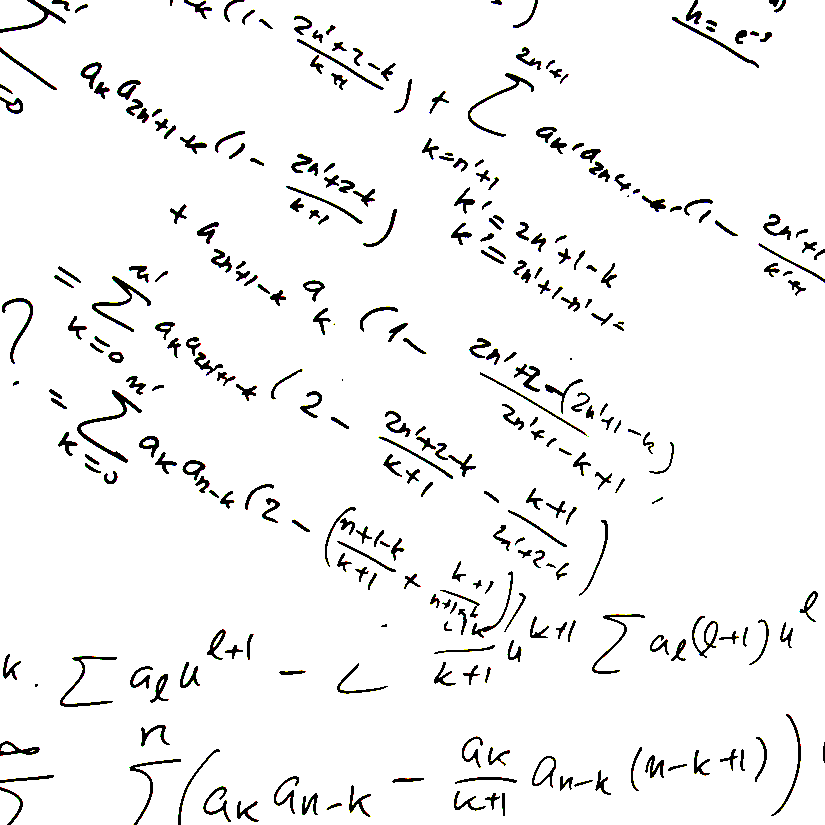
\includegraphics[width=8cm]{titlepic.png}
	};
\end{tikzpicture}
}

\usepackage[math]{iwona}

\newcommand{\hplus}{\mathbin{\hat+}}
\newcommand{\hdot}{\mathbin{\hat\cdot}}
% Описание теорем
\newtheorem{theorem}{Теорема}
\newtheorem{seq}{Следствие}
%%

%\VKR
\LECT % можно ещё лекцию забацать.
%\REPORT % можно ещё лекцию забацать.

%\titlepicture{
%%	\begin{tikzpicture}[overlay]
%%			\draw[opacity=0.4]  (-0.3,1.8) node {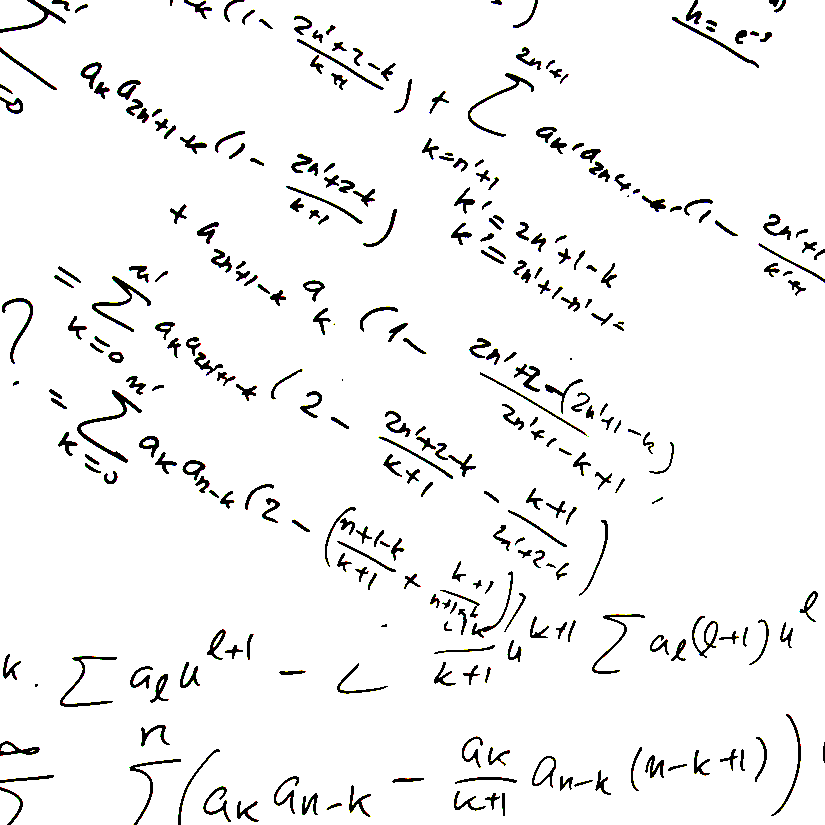
\includegraphics[width=3.5cm]{titlepic.png}};
%%	\end{tikzpicture}
%}

% Титульный лист теорем
\author[Д.\,В. Чупраков]{канд.\,физ.-матем.\,наук, доцент Д.\,В. Чупраков\\[6pt] usr10381@vyatsu.ru}

\institute[ВятГУ]{ФГБОУ ВО Вятский государственный университет}

\department{Факультет экономики и финансов}

\title[Лекция~3. Линейные задачи. Часть~1 из 4]{
	Введение в экономико-математическое моделирование\\[12pt]
	Лекция 3. Линейные задачи}
\subtitle{Матрицы. Определители. Системы линеных уравнений}


\date{22 cентября 2020 г.}


%\setbeamercolor{coloredboxstuff}{fg=yellow,bg=white!10!blue}

\setbeamercovered{invisible}


\tikzset{
	 myarrow/.style={->, >=latex', shorten >=1pt, thick}
}



\tikzset{add/.style n args={4}{
    minimum width=6mm,
    path picture={
        \draw[black] 
            (path picture bounding box.south east) -- (path picture bounding box.north west)
            (path picture bounding box.south west) -- (path picture bounding box.north east);
        \node at ($(path picture bounding box.south)+(0,0.13)$)     {\tiny #1};
        \node at ($(path picture bounding box.west)+(0.13,0)$)      {\tiny #2};
        \node at ($(path picture bounding box.north)+(0,-0.13)$)        {\tiny #3};
        \node at ($(path picture bounding box.east)+(-0.13,0)$)     {\tiny #4};
        }
    }
}

\tikzset{bigadd/.style n args={4}{
    minimum width=20mm,
    path picture={
        \draw[black] 
            (path picture bounding box.south east) -- (path picture bounding box.north west)
            (path picture bounding box.south west) -- (path picture bounding box.north east);
        \node at ($(path picture bounding box.south)+(0,0.5)$)     { #1};
        \node at ($(path picture bounding box.west)+(0.5,0)$)      {#2};
        \node at ($(path picture bounding box.north)+(0,-0.5)$)        {#3};
        \node at ($(path picture bounding box.east)+(-0.5,0)$)     {#4};
        }
    }
}
\begin{document}


\maketitle

\begin{frame}{Структура лекции}
	\tableofcontents
\end{frame}


%\section{Экономические задачи, приводящие к понятию матриц}

\section{Матрицы}
\subsection{Что такое матрица}
\begin{frame}{Матрицы. Основные понятия}
	\begin{block}{Определение}
		Прямоугольная таблица элементов какого-либо множества, имеющая $m$~строк и $n$~столбцов называется \alert{матрицей}.
	\end{block}

	\bigskip
	\structure{Обозначение}	
	$$
	A = \begin{pmatrix}
				a_{11} & a_{12} & \ldots & a_{1n} \\
				a_{21} & a_{22} & \ldots & a_{2n} \\
				\ldots & \ldots & \ldots &\ldots \\
				a_{m1} & a_{m2} & \ldots & a_{mn}
			\end{pmatrix} = (a_{ij})_{m \times n}.
	$$

	\bigskip
	\structure{Размерность матрицы:} $\dim A = (m\times n)$
\end{frame}

\begin{frame}{Виды матриц}
	\begin{description}
	\item[$m=1$:] 
		\alert{матрица-строка}~---
		$A = \begin{pmatrix}
			a_1 & a_2 & \ldots & a_n
		\end{pmatrix}$.
	\item[$n=1$:]
		\alert{матрица-столбец}~---
		$A = \begin{pmatrix} 
			a_1 \\ a_2 \\ \ldots \\ a_m 
		\end{pmatrix}$.
	\item[$n=m$:] 
		\alert{квадратная} матрица~---
		$A = \begin{pmatrix}
			a_{11} & a_{12} & \ldots & a_{1n} \\
			a_{21} & a_{22} & \ldots & a_{2n} \\
			\ldots & \ldots & \ldots &\ldots \\
			a_{n1} & a_{n2} & \ldots & a_{nn}
		\end{pmatrix}$.
		$n$~--- порядок квадратной матрицы $n\times n$.
	\item[$n\neq m$:] 
		\alert{прямоугольная} матрица.		
	\end{description}
\end{frame}

\begin{frame}{Специальные виды матриц}
\begin{minipage}{0.45\textwidth}
{\centering \alert{Квадратные}\par}
	\structure{Треугольная:}\\
		$A = \begin{pmatrix}
			a_{11} & a_{12} & \ldots & a_{1n} \\
			0 & a_{22} & \ldots & a_{2n} \\
			\ldots & \ldots & \ldots &\ldots \\
			0 & 0 & \ldots & a_{nn}
		\end{pmatrix}$.

	\medskip
	\structure{Диагональная:}\\
		$A = \begin{pmatrix}
			a_{11} & 0 & \ldots & 0 \\
			0 & a_{22} & \ldots & 0 \\
			\ldots & \ldots & \ldots &\ldots \\
			0 & 0 & \ldots & a_{nn}
		\end{pmatrix}$.

	\medskip
	\structure{Единичная:}\\
		$E = \begin{pmatrix}
			1 & 0 & \ldots & 0 \\
			0 & 1 & \ldots & 0 \\
			\ldots & \ldots & \ldots &\ldots \\
			0 & 0 & \ldots & 1
		\end{pmatrix}$.

\vfill
\end{minipage}\hfill
\begin{minipage}{0.45\textwidth}
{\centering \alert{Прямоугольные}\par}
	\structure{Нулевая:}\\
		$O_{m\times n} = \begin{pmatrix}
			0 & 0 & \ldots & 0 \\
			0 & 0 & \ldots & 0 \\
			\ldots & \ldots & \ldots &\ldots \\
			0 & 0 & \ldots & 0
		\end{pmatrix}$.		
	\vspace{5cm}
\end{minipage}
\end{frame}

\begin{frame}{Равенство матриц}
	\begin{block}{Равенство матриц}
		Матрицы \alert{равны}, если:
		\begin{itemize}
		\item 
			они имеют одинаковую размерность;
		\item
		 	их соответствующие элементы равны.
		\end{itemize} 
	\end{block}
	$$
	A_{n\times m} = B_{n'\times m'} \Longleftrightarrow 
	\left\lbrace
	\begin{aligned}
		n &= n'\\
		m &= m'\\
		a_{i,j} &=b_{i,j}\\
	\end{aligned}
	\right.
	$$

	\begin{exampleblock}{Применение}
		Метод неопределенных коэффициентов
	\end{exampleblock}

\end{frame}
\subsection{Линейные операции над матрицами}


\begin{frame}{Линейные операции матриц}
	\begin{block}{Сумма матриц}
		Сумма матриц определена только для матриц одинакового размера.
		При нахождении суммы соответствующие элементы матриц складываются. 
	\end{block}
	\vspace{-3mm}
	$$
	C = A + B \Longleftrightarrow 
	\left\lbrace\begin{aligned}
		\dim C &= \dim A =\dim B\\
		c_{i,j} &= a_{i,j} + b_{i,j}\\
	\end{aligned}
	\right.
	$$
	\begin{block}{Умножение матрицы на число}
		Результатом умножения матрицы~$A$ на число~$k$ является матрица того же размера, каждый элемент которой получается умножением соответствующего элемента матрицы~$A$  на~$k$.
	\end{block}	
	\vspace{-3mm}
		$$
		C = kA \Longleftrightarrow 
		\left\lbrace\begin{aligned}
			\dim C &= \dim A\\
			c_{i,j} &= k\cdot a_{i,j}\\
		\end{aligned}
		\right.
		$$
\end{frame}

\begin{frame}{Примеры}
	\structure{Найти значение выражения:}
	$$
		C=5A+B,\quad 
		A=\begin{pmatrix}
			1 & 3& 2\\
			0 & -1 & 4\\	
		\end{pmatrix},\quad
		B=\begin{pmatrix}
			2 & -4& 1\\
			-5 & 0 & 2\\	
		\end{pmatrix}
	$$	
	$$
		C
		=\begin{pmatrix}
			5\cdot 1+2 & 5\cdot 3 -4 & 5\cdot 2 + 1\\
			5\cdot 0 -5 & 5\cdot(-1)+0 & 5\cdot 4 + 2\\	
		\end{pmatrix}
		=\begin{pmatrix}
			7 & 11 & 11\\
			-5 & -5 & 22\\	
		\end{pmatrix}
	$$	
\end{frame}

\begin{frame}{Транспонирование матрицы}

	\begin{block}{}
		\alert{Транспонирование матрицы}~--- это операция над матрицей, при которой ее строки и столбцы меняются местами:
		$$
		(a_{ij})^T_{m\times n} = (a_{ji})_{n\times m} 
		$$
	\end{block}
\structure{Пример:}
$$
\begin{pmatrix}
1 & 2 & 3 \\
4 & 5 & 6 \\
\end{pmatrix}^T=
\begin{pmatrix}
1 & 4 \\
2 & 5 \\
3 & 6 \\
\end{pmatrix}
$$

\structure{Связь с линейными операциями:}
\begin{itemize}
%\item 
%	Если матрица A имеет размер $m \times n$, то транспонированная матрица $A^T$ имеет размер $n \times m$
\item 
    $(A^T)^T = A$
\item 
    $(kA)^T = kA^T$
\item 
    $(A + B)^T = A^T + B^T$
\end{itemize}
\end{frame}

\subsection{Умножение матриц}

\begin{frame}[fragile]{Умножение матриц}
%Произведение матриц~$A\times B$ определено только тогда, когда число столбцов матрицы~$A$ равно числу строк матрицы~$B$.

\begin{block}{Определение}
Произведением матриц~$A\times B$ называется матрица~$C$, если
\begin{itemize}
\item 
	$\dim A = (m\times n)$, $\dim B = (n\times k)$
\item 
	$\dim C = (m\times k)$
\item 
	$c_{ij} = A_i\cdot B^j= a_{i1}b_{1j}+a_{i2}b_{2j}+a_{i3}b_{3j}+\ldots+a_{in}b_{nj}$
\end{itemize}
\end{block}

\structure{Правило размерностей:}

{\centering
\begin{tikzpicture}[>=latex]
\matrix [matrix of math nodes,
	column 2/.style={nodes={circle,fill=vgured!40}},
	column 14/.style={nodes={circle,fill=vgured!40}},
%	column 4/.style={nodes={circle,fill=vgublue!40}},
%	column 8/.style={nodes={circle,fill=vgublue!40}},
	column 10/.style={nodes={circle,fill=vgugreen!40}},
	column 16/.style={nodes={circle,fill=vgugreen!40}},
]
(A) {
( &m   & \times &n  & ) & \cdot & (&n&\times & k &)& =&( & m &\times & k &)\\
};
\draw[->] (A-1-2)  to[out=-60, in=-120] (A-1-14);
\draw[->] (A-1-10)  to[out=60, in=120] (A-1-16);
\draw[double distance=1pt] (A-1-4)  to[out=60, in=120] (A-1-8);

\end{tikzpicture}
\par}
\end{frame}

\begin{frame}[fragile]{Схема умножения матриц}{}

\centering
\begin{tikzpicture}[
mymatrix/.style={
  matrix of math nodes,
  outer sep=0pt,
  nodes={
    draw,
    text width=2.5em,
    align=center,
    minimum height=2.5em,
    text=gray
  },
  nodes in empty cells,
  column sep=-\pgflinewidth,
  row sep=-\pgflinewidth,
  left delimiter=(,
  right delimiter=),
  },
  mycircle/.style 2 args={
    draw=#1,
    circle,
    fill=#2,
    line width=2pt,
    inner sep=5pt
  },
  arr/.style={
  line width=4pt,
  -{Triangle[angle=60:1.5pt 3]},
  #1,
  shorten >= 3pt,
  shorten <= 3pt
  }
]
%the matrices
\matrix[mymatrix] (A)
{
|[text=black]|a_{11} & |[text=black]|a_{12} \\
a_{21} & a_{22} \\
|[text=black]|a_{31} & |[text=black]|a_{32} \\
a_{41} & a_{42} \\
};
\matrix[mymatrix,right=of A.north east,anchor=north west] (prod)
{
& & \\
& & \\
& & \\
& & \\
};
\matrix[mymatrix,above=16pt of prod.north west,anchor=south west] (B)
{
b_{11} & |[text=black]|b_{12} & |[text=black]|b_{13} \\
b_{21} & |[text=black]|b_{22} & |[text=black]|b_{23} \\
};

%the labels for the matrices
\node[font=\huge,left=10pt of A] {$A$};
\node[font=\huge,left=10pt of B] {$B$};

%the frames in both matrices
\draw[vgured,line width=2pt]
  ([shift={(1.2pt,-1.2pt)}]A-1-1.north west) 
  rectangle 
  ([shift={(-1.2pt,1.2pt)}]A-1-2.south east);
\draw[cyan,line width=2pt]
  ([shift={(1.2pt,-1.2pt)}]B-1-2.north west) 
  rectangle 
  ([shift={(-1.2pt,1.2pt)}]B-2-2.south east);
\draw[vgublue,line width=2pt]
  ([shift={(1.2pt,-1.2pt)}]A-3-1.north west) 
  rectangle 
  ([shift={(-1.2pt,1.2pt)}]A-3-2.south east);
\draw[vgugreen,line width=2pt]
  ([shift={(1.2pt,-1.2pt)}]B-1-3.north west) 
  rectangle 
  ([shift={(-1.2pt,1.2pt)}]B-2-3.south east);

%the filled circles in the product
\node[mycircle={vgublue}{vgugreen}]
  at (prod-3-3) (prod33) {};
\node[mycircle={vgured}{cyan}]
  at (prod-1-2) (prod12) {};

%the arrows
\draw[arr=vgured]
  (A-1-2.east) -- (prod12); 
\draw[arr=cyan]
  (B-2-2.south) -- (prod12); 
\draw[arr=vgublue]
  (A-3-2.east) -- (prod33); 
\draw[arr=vgugreen]
  (B-2-3.south) -- (prod33); 

%the legend
\matrix[
  matrix of math nodes,
  nodes in empty cells,
  column sep=10pt,
  anchor=north,
  nodes={
    minimum height=2.2em,
    minimum width=2em,
    anchor=north west
  },
  below=5pt of current bounding box.south
  ] 
  (legend)
{
  & a_{11}b_{12} + a_{12}b_{22} & & & a_{31}b_{13} + a_{32}b_{23} \\
};
\node[mycircle={vgublue}{vgugreen}]
  at (legend-1-4) {};
\node[mycircle={vgured}{cyan}]
  at (legend-1-1) {};
\draw[dashed,lightgray] (A-1-1) |- (B-1-1);
\draw[dashed,lightgray] (A-1-2) |- (B-2-1);
\end{tikzpicture}
\end{frame}
\begin{frame}[allowframebreaks]{Пример умножения матриц}{}
	\begin{exampleblock}{Задача}
		Вычислить:
		$\begin{pmatrix}3&5\\6&-1\end{pmatrix} \cdot \begin{pmatrix}2&1 & 0\\-3&2 & 1\end{pmatrix}$.
	\end{exampleblock}
	\begin{itemize}
	\item 
		Размерность $(2\times 2)$, $(2\times 3)$. Умножать можно. Произведение $2 \times 3$

	\item 
		$\begin{pmatrix}3&5\\6&-1\end{pmatrix} \cdot \begin{pmatrix}2&1 & 0\\-3&2 & 1\end{pmatrix}
		= \begin{pmatrix}c_{11}& c_{12} & c_{13}\\ c_{21} &c_{22} & c_{23}\end{pmatrix}$
	\framebreak
	\item Вычисляем элементы:
		\begin{itemize}
		\item[$\bullet$]
			 $c_{11} =  \begin{pmatrix}3 & 5 \end{pmatrix} \cdot \begin{pmatrix}2\\-3\end{pmatrix} = 2\cdot 3+5\cdot(-3)=-9$
		\item[$\bullet$] 
			 $c_{12} =  \begin{pmatrix}3 & 5 \end{pmatrix} \cdot \begin{pmatrix}1\\2\end{pmatrix} = 2\cdot 1+5\cdot 2=12$
		\item[$\bullet$]
			 $c_{13} =  \begin{pmatrix}3 & 5 \end{pmatrix} \cdot \begin{pmatrix}0\\1\end{pmatrix} = 2\cdot 0+5\cdot 1=5$

		\item[$\bullet$] 
			 $c_{21} =  \begin{pmatrix}6 & -1 \end{pmatrix} \cdot \begin{pmatrix}2\\-3\end{pmatrix} = 6\cdot 3+(-1)\cdot(-3)=21$
		\item[$\bullet$] 
			 $c_{22} =  \begin{pmatrix}6 & -1 \end{pmatrix} \cdot \begin{pmatrix}1\\2\end{pmatrix} = 6\cdot 1+(-1)\cdot 2=4$
		\item[$\bullet$] 
			 $c_{23} =  \begin{pmatrix}6 & -1 \end{pmatrix} \cdot \begin{pmatrix}0\\1\end{pmatrix} = 6\cdot 0+(-1)\cdot 1=-1$
		 \end{itemize}
	\item 
	Итак,
		$\begin{pmatrix}3&5\\6&-1\end{pmatrix} \cdot \begin{pmatrix}2&1 & 0\\-3&2 & 1\end{pmatrix}
		= \alert{\begin{pmatrix}-9 & 12 & 5\\ 21 & 4 & -1\end{pmatrix}}$		
	\end{itemize}
\begin{alertblock}{}
Заметим, что 
$
\begin{pmatrix}2&1 & 0\\-3&2 & 1\end{pmatrix}\cdot\begin{pmatrix}3&5\\6&-1\end{pmatrix}
$ не существует, так как число столбцов первого множителя не равно числу строк второго множителя. 

\end{alertblock}
\end{frame}

\begin{frame}[allowframebreaks]{Умножение матриц в экономике}{}
\begin{exampleblock}{Задача}
В таблице указана стоимость доставки единицы продукции, отгружаемой ежедневно на молокозаводах~1 и~2 в магазины $M_1$, $M_2$ и $M_3$. Подсчитать ежедневные транспортные расходы каждого завода, если  с каждого молокозавода в магазин $M_1$ доставляют по 50 ед. продукции, в~магазин~$M_2$~--- по 70, а~в~$M_3$~--- по 130 ед. продукции.

{\centering
\begin{tabular}{cccc}
\hline
& \multicolumn{3}{c}{Магазины}\\
Молокозавод & $M_1$ & $M_2$ & $M_3$\\
\hline
1 & 20 & 35 & 10\\
2 & 15 & 27 & 8\\
\hline
\end{tabular}
\par
}
\end{exampleblock}

Обозначим через $A$ матрицу, характеризующую стоимость доставки
единицы продукции в магазины,  а через $B$~--- матрицу количества единиц продукции:
$$
A = \begin{pmatrix}
20 & 35 & 10 \\ 15 & 27 & 8\\
\end{pmatrix},
B = \begin{pmatrix}
50 \\ 70 \\ 130
\end{pmatrix}
$$

\begin{multline*}
AB  = \begin{pmatrix}
20 & 35 & 10 \\ 15 & 27 & 8\\
\end{pmatrix}\cdot \begin{pmatrix}
50 \\ 70 \\ 130
\end{pmatrix}
=\\
=
\begin{pmatrix}
20 \cdot 50 + 35 \cdot 70 + 10\cdot 130 \\ 15\cdot 50 + 27\cdot 70 + 8\cdot 130\\
\end{pmatrix}
=
\begin{pmatrix}
4750 \\3680\\
\end{pmatrix}
\end{multline*}

Задача решена, однако, если мы домножим $AB$ на матрицу, характеризующую распределение поставок между молокозаводами $C=\begin{pmatrix}
1 & 1
\end{pmatrix}$, то  получим суммарную стоимость доставки: 
$$
CAB = \begin{pmatrix}
1 & 1
\end{pmatrix} \cdot 
\begin{pmatrix}
4750 \\3680\\
\end{pmatrix}
=(8430)
$$

\hrule
\medskip

Итак, на доставку товаров тратится 8430 руб ежедневно, причем 4750 руб. стоит доставка с первого завода и 3680~--- со~второго.
\end{frame}

\begin{frame}{Свойства умножения  матрицами}{}

\begin{itemize}
\item $A(BC)=(AB)C$
\item $k(AB)=(kA)B=A(kB)$
\item $(A+B)C=AC+BC$,\quad $A(B+C)=AB+AC$
\item[\alert{$\blacktriangleright$}] \alert{$AB\neq BA$} 
\item $(AB)^T=B^TA^T$
\item $A_{m\times n}E_{n\times n} =A_{m\times n}$, $E_{m\times m}A_{m\times n} = A_{m\times n}$
\item $AE = EA=E$, если $A$~--- квадратная матрица.
\end{itemize}
\begin{block}{Определение}
Матрицы $A$ и~$B$ называются \alert{перестановочными}, если $AB = BA$. 
\end{block}
\end{frame}

\begin{frame}[allowframebreaks]{Проблема деления матриц}
\begin{itemize}
\item Попробуем ,,разделить`` $\begin{pmatrix} 1 & 1 \\ 1 & 0 \end{pmatrix}$ на $\begin{pmatrix} 1 & 2 \\ 3 & 5 \end{pmatrix}$.

Для этого решим уравнение
$
\begin{pmatrix} 1 & 2 \\ 3 & 5 \end{pmatrix}
\begin{pmatrix} a & b \\ c & d \end{pmatrix} = \begin{pmatrix} 1 & 1 \\ 1 & 0 \end{pmatrix}
$

Перемножим
$
\begin{pmatrix} a+2c & b+2d \\ 3a+5c & 3b+5d \end{pmatrix} = \begin{pmatrix} 1 & 1 \\ 1 & 0 \end{pmatrix}
$

По определению равенства матриц:
$$
\left\lbrace\begin{aligned}
	a+2c &= 1\\
	b+2d &=1\\
	3a+5c &=1\\
	3b+5d &=0\\
\end{aligned}
\right.
\Longleftrightarrow
\left\lbrace\begin{aligned}
	a &= 3\\
	b &= -10/3\\
	c &= 2\\
	d &= 13/6\\
\end{aligned}
\right.
$$
Итак,
$$
\begin{pmatrix} 1 & 2 \\ 3 & 5 \end{pmatrix}
\alert{\begin{pmatrix} 3 & -10/3 \\ 2 & 13/6 \end{pmatrix}} = \begin{pmatrix} 1 & 1 \\ 1 & 0 \end{pmatrix}
$$

\item 
	Попробуем теперь ,,разделить`` $\begin{pmatrix} 1 & 1 \\ 1 & 0 \end{pmatrix}$ на $\begin{pmatrix} 1 & 1 \\ 1 & 1 \end{pmatrix}$.

$$
\begin{gathered}
	\begin{pmatrix} 
		1 & 1 \\ 
		1 & 1 
	\end{pmatrix}
	\begin{pmatrix} 
		a & b \\ 
		c & d 
	\end{pmatrix} 
	= 
	\begin{pmatrix} 
		1 & 1 \\ 
		1 & 0
	\end{pmatrix}
	\\\Updownarrow
	\\
	\begin{pmatrix} 
		a+c & b+d \\ 
		a+c & b+d 
	\end{pmatrix} 
	= 
	\begin{pmatrix} 
		1 & 1 \\ 
		1 & 0 
	\end{pmatrix}
	\\\Updownarrow
	\\
\left\lbrace\begin{aligned}
	a+c &= 1\\
	b+d &=1\\
	a+c &=1\\
	b+d &=0\\
\end{aligned}
\right. \Longrightarrow 0=b+d=1
\end{gathered}
$$
\alert{Таким образом, операция деления матриц не определена.}
\end{itemize}

\end{frame}

\begin{frame}{Определение определителя}{}
Каждой квадратной матрице сопоставляется число, называемое \alert{определителем}, по следующим правилам: 
\begin{enumerate}
\item 
\alert{Определитель матрицы первого порядка} равен его единственному элементу:
\hfill
	$
	A= \begin{pmatrix}
		a_{11}
	\end{pmatrix} 
	\Longrightarrow  \det(A) = a_{11}.
	$
	
\item 
	\alert{Определитель матрицы $n$-го порядка} равен сумме произведений элементов его первой строки на~соответствующие им алгебраические дополнения:
	$$
	\det(A)=\left|~\begin{matrix}
			\rowcolor{vgured!20} a_{11} & a_{12} & \ldots & a_{1n} \\
			a_{21} & a_{22} & \ldots & a_{2n} \\
			\ldots & \ldots & \ldots &\ldots \\
			a_{n1} & a_{n2} & \ldots & a_{nn}
		\end{matrix}~\right| = a_{11}A_{11}+ a_{12}A_{12}+ \ldots + a_{1n}A_{1n},
	$$
где
\item[$\blacktriangleright$] 
	$A_{ij}=(-1)^{i+j}M_{ij}$~--- \alert{алгебраическое дополнение};
\item[$\blacktriangleright$]
	$M_{ij}$~--- \alert{минор элемента~$a_{ij}$}~--- определитель матрицы, полученной из $A$ вычеркиванием $i$-й строки и $j$-го столбца.
\end{enumerate}
\end{frame}

\section{Определитель}
\subsection{Определение определителя}
\begin{frame}[fragile]{Определитель второго порядка}{}
\begin{block}{Теорема}
\itshape
Определителем матрицы второго порядка  является число
$
	\begin{vmatrix}
	a_1 & b_1 \\
	a_2 & b_2 \\
	\end{vmatrix} =  {\color{red} a_1b_2} {\color{blue}{} -b_1a_2}. 
$
\end{block}

	\structure{Правило вычисления:}\quad
	\begin{tikzpicture}[
		baseline,
		>=latex,
	]
	\matrix (mtrx) [
		matrix of math nodes,
		column sep=0ex,   
		nodes={text height=2ex,text width=2ex}
	]
	{
	|[vgured]|+ & a_1 & b_1 &  \\
	|[vgublue]|- &a_2 & b_2 & \\
	};

	\draw[thick,rounded corners=6pt] 
		(mtrx-1-2.north west) -- (mtrx-2-2.south west);
	\draw[thick,rounded corners=6pt] 
		(mtrx-1-3.north east)--(mtrx-2-3.south east);
	\path[
			draw,
			vgured,
			very thick,
			opacity=0.6,
			->
		]	    
	    (mtrx-1-2.north west) -- (mtrx-2-3.south east);
	\path[
			draw,
			vgublue ,
			very thick,
			opacity=0.6,
			->
		]	    
		(mtrx-2-2.south west) -- (mtrx-1-3.north east);
	\end{tikzpicture}

\bigskip

\structure{Доказательство.}
Разложим определитель по первой строке.
	$
		\begin{vmatrix}
		a_1 & b_1 \\
		a_2 & b_2 \\
		\end{vmatrix} 
		=  a_1 (-1)^{1+1}M_{11} + b_1 (-1)^{1+2}M_{12}
		=  a_1 b_2 - b_1 a_2
	$
	
\end{frame}

\begin{frame}[fragile]{Определитель третьего порядка}{}
\begin{block}{Теорема}
\itshape
Определителем матрицы третьего порядка  является число
{\small
$
	\begin{vmatrix}
	a_1 & b_1 & c_1 \\
	a_2 & b_2 & c_2 \\
	a_3 & b_3 & c_3 \\
	\end{vmatrix} =  {\color{red} a_1b_2c_3 + b_1c_2a_3 + c_1a_2b_3} {\color{blue}{} -a_3b_2c_1 - b_3c_2a_1 - c_3a_2 b_1 }. 
$\par}
\end{block}

\vspace{-2mm}
\structure{Правило Саррюса:}\quad
	\begin{tikzpicture}[
		baseline,
		>=latex,
	]
	\matrix (mtrx) [
		matrix of math nodes,
		column sep=1ex,   
		nodes={text height=2ex,text width=2ex}
	]
	{
	|[vgured]|+ & |[vgured]|+ & |[vgured]|+ & &\\
	a_1 & b_1 & c_1 & |[gray]| a_1 & |[gray]| b_1   \\
	a_2 & b_2 & c_2 & |[gray]| a_2 & |[gray]| b_2   \\
	a_3 & b_3 & c_3 & |[gray]| a_3 & |[gray]| b_3   \\
	|[vgublue]|- & |[vgublue]|- & |[vgublue]|-& &  \\
	};
%%	\node[right= 1mm of mtrx]{$=$};
%
%%	\node[below right= 1mm of mtrx.south west]
%%	{$= {\color{red} a_1b_2c_3 + b_1c_2a_3 + c_1a_2b_3} {\color{blue}{} -a_3b_2c_1 - b_3c_2a_1 - c_3a_2 b_1 } $};

	\draw[thick,rounded corners=6pt] 
		(mtrx-2-1.north west) -- (mtrx-4-1.south west);
	\draw[thick,rounded corners=6pt] 
		(mtrx-2-3.north east)--(mtrx-4-3.south east);
	\path[
		draw,
		vgublue ,
		very thick,
		opacity=0.6,
		->
	]	    
		(mtrx-4-1.south west) edge (mtrx-2-3.north east)
	    (mtrx-4-2.south west) edge (mtrx-2-4.north east)
	    (mtrx-4-3.south west)  --  (mtrx-2-5.north east);
	\path[
		draw,
		vgured,
		very thick,
		opacity=0.6,
		->
	]
	    (mtrx-2-1.north west) edge (mtrx-4-3.south east)
	    (mtrx-2-2.north west) edge (mtrx-4-4.south east)
	    (mtrx-2-3.north west)  --  (mtrx-4-5.south east);
	\end{tikzpicture}

\bigskip
\alert{Внимание!}
	Правило Саррюса применяется только для определителей 3 порядка.
\end{frame}
\begin{frame}[allowframebreaks,fragile]{Примеры вычисления определителя}
\begin{itemize}
\item 
	Определитель второго порядка:
	
	\begin{tikzpicture}[
		baseline,
		>=latex,
	]
	\matrix (mtrx) [
		matrix of math nodes,
		column sep=0ex,   
		nodes={text height=2ex,text width=2ex,align=center}
	]
	{
	 & -1 & 4 &  \\
	 &-5 & 2 & \\
	};

	\draw[thick,rounded corners=6pt] 
		(mtrx-1-2.north west) -- (mtrx-2-2.south west);
	\draw[thick,rounded corners=6pt] 
		(mtrx-1-3.north east)--(mtrx-2-3.south east);
	\path[
			draw,
			vgured,
			very thick,
			opacity=0.6,
			->
		]	    
	    (mtrx-1-2.north west) -- (mtrx-2-3.south east);
	\path[
			draw,
			vgublue ,
			very thick,
			opacity=0.6,
			->
		]	    
		(mtrx-2-2.south west) -- (mtrx-1-3.north east);
	\end{tikzpicture}
	$ = (-1)\cdot 2 - (-5)\cdot 4 = 18$.
\item 
	Определитель третьего порядка:
	${\begin{vmatrix}
		-6 & 5  & 0  \\
		0  & -6 & -2 \\
		3  & 2  & 2
	\end{vmatrix}}=$\begin{tikzpicture}[
		baseline,
		>=latex,
	]
	\matrix (mtrx) [
		matrix of math nodes,
		column sep=1ex,   
		nodes={text height=2ex,text width=2ex,align=center}
	]
	{
	|[vgured]|+ & |[vgured]|+ & |[vgured]|+ & &\\
	-6 &  5 &  0 &|[gray]| -6 &|[gray]|  5\\
	 0 & -6 & -2 &|[gray]|  0 &|[gray]| -6\\
	 3 &  2 &  2 &|[gray]|  3 &|[gray]|  2\\
	|[vgublue]|- & |[vgublue]|- & |[vgublue]|-& &  \\
	};
	\draw[thick,rounded corners=6pt] 
		(mtrx-2-1.north west) -- (mtrx-4-1.south west);
	\draw[thick,rounded corners=6pt] 
		(mtrx-2-3.north east)--(mtrx-4-3.south east);
	\path[
		draw,
		vgublue ,
		very thick,
		opacity=0.6,
		->
	]	    
		(mtrx-4-1.south west) edge (mtrx-2-3.north east)
	    (mtrx-4-2.south west) edge (mtrx-2-4.north east)
	    (mtrx-4-3.south west)  --  (mtrx-2-5.north east);
	\path[
		draw,
		vgured,
		very thick,
		opacity=0.6,
		->
	]
	    (mtrx-2-1.north west) edge (mtrx-4-3.south east)
	    (mtrx-2-2.north west) edge (mtrx-4-4.south east)
	    (mtrx-2-3.north west)  --  (mtrx-4-5.south east);
	\end{tikzpicture}$=$
	$= {\color{vgured} 72-30+0}  {\color{vgublue}{} -0-24-0}= 18$.
	
\framebreak
\item 
	Определитель четвертого порядка:
	$\begin{vmatrix}
		0 & 1 & 2  & 0  \\
		1 & 0 & 1  & 6  \\
		1 & 1 & 0  & -2 \\
		3 & 6 & -2 & 0
	\end{vmatrix} = 0A_{11}+A_{12}+2A_{13}+0A_{14}
	$
	\begin{itemize}
	\item[$\bullet$] $A_{12}=(-1)^{1+2}$
		\begin{tikzpicture}[
			baseline,
			>=latex,
		]
		\matrix (mtrx) [
			matrix of math nodes,
			column sep=1ex,   
			nodes={text height=2ex,text width=2ex,align=center}
		]
		{
			0 & 1 & 2  & 0  \\
			1 & 0 & 1  & 6  \\
			1 & 1 & 0  & -2 \\
			3 & 6 & -2 & 0 \\
		};
		\draw[thick] 
			(mtrx-1-1.north west) -- (mtrx-4-1.south west)
			(mtrx-1-4.north east)--(mtrx-4-4.south east);
		\draw[thick, vgured] 
			(mtrx-1-2.north) --  (mtrx-4-2.south)
			(mtrx-1-1.west) -- (mtrx-1-4.east);
		\end{tikzpicture}
		$=-\begin{vmatrix}
			1 &  1  & 6  \\
			1 &  0  & -2 \\
			3 &  -2 & 0\\
		\end{vmatrix}=$
		
		\hfill$= -({\color{vgured} 0-6-12}  {\color{vgublue}{} -0-4-0})= 22$
	\item[$\bullet$] $A_{13}=(-1)^{1+3}$
		\begin{tikzpicture}[
			baseline,
			>=latex,
		]
		\matrix (mtrx) [
			matrix of math nodes,
			column sep=1ex,   
			nodes={text height=2ex,text width=2ex,align=center}
		]
		{
			0 & 1 & 2  & 0  \\
			1 & 0 & 1  & 6  \\
			1 & 1 & 0  & -2 \\
			3 & 6 & -2 & 0 \\
		};
		\draw[thick] 
			(mtrx-1-1.north west) -- (mtrx-4-1.south west)
			(mtrx-1-4.north east)--(mtrx-4-4.south east);
		\draw[thick, vgured] 
			(mtrx-1-3.north) --  (mtrx-4-3.south)
			(mtrx-1-1.west) -- (mtrx-1-4.east);
		\end{tikzpicture}
		$=\begin{vmatrix}
			1 & 0 & 6  \\
			1 & 1 & -2 \\
			3 & 6 & 0 \\
		\end{vmatrix}=$
		
		\hfill$= {\color{vgured} 0-0+36}  {\color{vgublue}{} -18+12-0} = 30$
		
		\bigskip
		\item[$\bullet$] Подставим алгебраические дополнения в разложение определителя:
		
			$\begin{vmatrix}
				0 & 1 & 2  & 0  \\
				1 & 0 & 1  & 6  \\
				1 & 1 & 0  & -2 \\
				3 & 6 & -2 & 0
			\end{vmatrix} = 18+2\cdot 30 =78
			$
		\end{itemize}
	
\end{itemize}
\end{frame}
\subsection{Свойства определителя}
\begin{frame}[allowframebreaks]{Свойства определителя}{}
	\begin{enumerate}
	\item 
	    Определитель может быть разложен в линейную комбинацию по любой строке и любому столбцу.
	\item 
	    Определитель транспонированной матрицы равен определителю исходной матрицы:
   
	    \hfill
	    \alert{$
		\begin{vmatrix}
			1 & 2\\
			3 & 4
		\end{vmatrix} 
		=
		\begin{vmatrix}
			1 & 3\\
			2 & 4
		\end{vmatrix} 
		$}
	\item 
	    Умножение всех элементов строки или столбца определителя на некоторое число $\lambda$ равносильно умножению определителя на это число:
    
	    \hfill
		\alert{$
		\begin{vmatrix}
			1 & 2\\
			3 & 4
		\end{vmatrix} 
		= 
		2\begin{vmatrix}
			1 & 1\\
			3 & 2
		\end{vmatrix} 
		$}

	\item 
	    Если в определителе переставить местами любые две строки или два столбца, то определитель изменяет свой знак на противоположный.
    
	    \hfill
		\alert{$
		\begin{vmatrix}
			1 & 2\\
			3 & 4
		\end{vmatrix} 
		= 
		-\begin{vmatrix}
			3 & 4\\
			1 & 2\\
		\end{vmatrix} 
		$}
	
	\item 
	    Если матрица содержит \alert{нулевую строку} (столбец), то определитель этой матрицы равен нулю.

	    \hfill
		\alert{$
		\begin{vmatrix}
			1 & 2\\
			0 & 0
		\end{vmatrix} 
		= 0
		$}
	\item 
		Если две строки (столбца) матрицы \alert{равны}, то определитель этой матрицы равен нулю:

	    \hfill
		\alert{$
		\begin{vmatrix}
			1 & 2\\
			1 & 2
		\end{vmatrix} 
		= 0
		$}


	\item 
		Если две строки (столбца) матрицы \alert{пропорциональны друг другу}, то определитель этой матрицы равен нулю:

	    \hfill
		\alert{$
		\begin{vmatrix}
			1 & 2\\
			4 & 8
		\end{vmatrix} 
		= 0
		$}

	\item 
	    Определитель не изменится, если к элементам любой его строки (или столбца) прибавить соответствующие элементы другой строки (или соответствующего столбца), умноженные на некоторое число:
	    
	    \hfill
		\alert{$
		\begin{vmatrix}
			1 & 2\\
			3 & 4
		\end{vmatrix} 
		\begin{matrix}
			\\
			+5\text{I}
		\end{matrix} 
		= 
		\begin{vmatrix}
			1 & 2\\
			3+5 & 4+10
		\end{vmatrix} 
		= 
		\begin{vmatrix}
			1 & 2\\
			8 & 14
		\end{vmatrix} 
		$}
		
	\item 
		 Если все элементы $k$-ой строки определителя представлены в виде сумм  $a_{kj} + b_{kj}$, то определитель можно представить в виде суммы определителей, 
		$k$-я строка которых состоит из элементов $a_{kj}$ и $b_{kj}$ соответственно:
		
	    \hfill
		\alert{$
		\begin{vmatrix}
			1 & 2\\
			2+1 & 5-1
		\end{vmatrix}
		= 
		\begin{vmatrix}
			1 & 2\\
			2 & 5
		\end{vmatrix}
		+
		\begin{vmatrix}
			1 & 2\\
			1 & -1
		\end{vmatrix}
		$}

	\item 
		Определитель треугольной матрицы  равен произведению элементов, стоящих на главной диагонали:

	    \hfill
		\alert{$
		\begin{vmatrix}
			1 & 2  & 3\\
			0 & 4  & 5\\
			0 & 0  & 6\\
		\end{vmatrix}
		= 1\cdot 4 \cdot 6
		$}

	\item 
    Пусть $A$ и $B$~--- квадратные матрицы одного и того же порядка. Тогда определитель произведения матриц равен произведению определителей.
	
	\hfill
	\alert{$
	\det(AB)=\det(A)\cdot \det(B)$}
\end{enumerate}


\end{frame}

\begin{frame}{Элементарные преобразования}
\begin{enumerate}
\item 
	К одной строке определителя прибавить другую строку, умноженную на некоторое число.
	
	\hfill\alert{Определитель не меняется}	
\item 
	Переставить две строки местами

	\hfill\alert{и поменять знак перед определителем}	
\item 
	Умножить строку на ненулевое число $\lambda$

	\hfill\alert{и перед определителем записать множитель $\frac{1}{\lambda}$}	
\end{enumerate}
\begin{block}{}
Любой определитель можно привести к треугольному виду, получив нули под диагональю. 
\end{block}
\end{frame}

\begin{frame}[allowframebreaks]{\largeВычисление определителя преобразованиями}{}
	\begin{exampleblock}{Задача}
		Вычислить определитель
		$
			\det{A}= \begin{vmatrix}1&2&3&4\\ 2&3&4&1\\ 3&4&1&2\\ 4&1&2&3\end{vmatrix}
		$
	\end{exampleblock}
\vspace{-5mm}
	\begin{multline*}
		\begin{array}{|cccc|}
			\cellcolor{vgured!50}1 & 2 & 3 & 4 \\
			2 & 3 & 4 & 1 \\
			3 & 4 & 1 & 2 \\
			4 & 1 & 2 & 3
		\end{array}
		\alert{\begin{matrix}
			\\
			-2I \\
			-3I\\
			-4I
		\end{matrix}}
		= \begin{vmatrix}
			1 & 2 & 3 & 4 \\
			2-2 & 3-4 & 4-6 & 1-8 \\
			3-3 & 4-6 & 1-9 & 2-12 \\
			4-4 & 1-8 & 2-12 & 3-16
		\end{vmatrix}
		=\\
		= \begin{array}{|>{\columncolor{gray!50}}cccc|}
			\rowcolor{gray!50}\cellcolor{vgublue!50}1 & 2 & 3 & 4 \\
			0 & \cellcolor{vgured!50}-1 & -2 & -7 \\
			0 & -2 & -8 & -10 \\
			0 & -7 & -10 & -13
		\end{array}
	\end{multline*}
	\framebreak
	\begin{align*}
		&= \begin{array}{|>{\columncolor{gray!50}}cccc|}
			\rowcolor{gray!50}\cellcolor{vgublue!50}1 & 2 & 3 & 4 \\
			0 & \cellcolor{vgured!50}-1 & -2 & -7 \\
			0 & -2 & -8 & -10 \\
			0 & -7 & -10 & -13
		\end{array}
		\alert{\begin{matrix}
			\\
			 \\
			-2II\\
			-7II
		\end{matrix}}
		= \begin{array}{|>{\columncolor{gray!50}}c>{\columncolor{gray!50}}ccc|}
			\rowcolor{gray!50}\cellcolor{vgublue!50}1 & 2 & 3 & 4 \\
			\rowcolor{gray!50}0 & \cellcolor{vgublue!50}-1 & -2 &  -7 \\
			0 &  0 & \cellcolor{vgured!50}-4 &   4 \\
			0 &  0 &  4 &  36 \\
		\end{array}
		\alert{\begin{matrix}
			\\
			 \\
			\\
			+III
		\end{matrix}}
		=\\
		&= \begin{array}{|>{\columncolor{gray!50}}c>{\columncolor{gray!50}}c>{\columncolor{gray!50}}cc|}
			\rowcolor{gray!50}\cellcolor{vgublue!50}1 & 2 & 3 & 4 \\
			\rowcolor{gray!50}0 & \cellcolor{vgublue!50}-1 & -2 &  -7 \\
			\rowcolor{gray!50}0 &  0 & \cellcolor{vgublue!50}-4 &   4 \\
			0 &  0 &  0 &  \cellcolor{vgured!50}40 \\
		\end{array}
		= 1 \cdot (-1) \cdot (-4) \cdot 40 = 160.
	\end{align*}
\end{frame}

\subsection{Обратная матрица}
\begin{frame}{Обратная матрица}{}
	\begin{block}{Определение}
		\alert{Обратной матрицей} $A^{-1}$ по~отношению к данной невырожденной квадратной матрице $n$-го порядка, называется матрица, которая, будучи умноженной как слева, так и справа на данную матрицу, дает единичную матрицу. 
	\end{block}
	$$
		AA^{-1}=A^{-1}A=E
	$$
	\begin{block}{Критерий существования обратной матрицы}
		\itshape
		Обратная матрица $A^{-1}$ существует тогда и только тогда, когда определитель матрицы $A$ не равен нулю.
	\end{block}
\end{frame}

\begin{frame}{Нахождение обратной матрицы}{}
\alert{Присоединенная матрица}~--- матрица, в которой вместо каждого элемента поставлено его алгебраическое дополнение, а затем матрица транспонирована
$$
A^*=\begin{pmatrix}
A_{11} & A_{12} & \cdots & A_{1n}\\
A_{21} & A_{22} & \cdots & A_{2n}\\
\cdots & \cdots & \cdots & \cdots\\
A_{n1} & A_{n2} & \cdots & A_{nn}\\
\end{pmatrix}^T.
$$

\begin{block}{Вычисление обратной матрицы}
$$
	\det(A) \neq 0 \qquad\longrightarrow\qquad	\alert{A^{-1}=\frac{1}{\det(A)}A^*}
$$
\end{block}
\end{frame}
\begin{frame}[allowframebreaks,fragile]{Пример нахождения обратной матрицы}{}
\begin{exampleblock}{Задача}
Найти обратную матрицу 
	к~$ A= \begin{pmatrix}
		0 & 3 & 1 \\
		2 & 4 & 1 \\
		2 & 2 & 0 \\
		\end{pmatrix}
	$, если она существует.
\end{exampleblock}

\bigskip
\begin{enumerate}
\item 
	 Найдем определитель:
	$$
	A= \begin{vmatrix}
			0 & 3 & 1 \\
			2 & 4 & 1 \\
			2 & 2 & 0 \\
		\end{vmatrix} = 0+6+4-8-0-0=2\neq 0.
	$$ 
	
	\alert{Обратная матрица существует!}
     \framebreak	
\item 
	Найдем алгебраические дополнения :
\begin{itemize}
\item
	$A_{11} = (-1)^{1+1} \begin{vmatrix} 4 & 1 \\ 2 & 0\end{vmatrix} = -2$
	\hfill
	\begin{tikzpicture}[
		baseline,
		>=latex,
	]
	\matrix (mtrx) [
		matrix of math nodes,
		column sep=1ex,   
		nodes={text height=2ex,text width=2ex,align=center}
	]
	{
		0 & 3 & 1 \\
		2 & 4 & 1 \\
		2 & 2 & 0 \\
	};
	\draw[thick] 
		(mtrx-1-1.north west) -- (mtrx-3-1.south west)
		(mtrx-1-3.north east)--(mtrx-3-3.south east);
	\draw[thick, vgured] 
		(mtrx-1-1.north) --  (mtrx-3-1.south)
		(mtrx-1-1.west) -- (mtrx-1-3.east);
	\end{tikzpicture}

\item
	$A_{12} = (-1)^{1+2} \begin{vmatrix} 2 & 1 \\ 2 & 0\end{vmatrix} = 2$
	\hfill
	\begin{tikzpicture}[
		baseline,
		>=latex,
	]
	\matrix (mtrx) [
		matrix of math nodes,
		column sep=1ex,   
		nodes={text height=2ex,text width=2ex,align=center}
	]
	{
		0 & 3 & 1 \\
		2 & 4 & 1 \\
		2 & 2 & 0 \\
	};
	\draw[thick] 
		(mtrx-1-1.north west) -- (mtrx-3-1.south west)
		(mtrx-1-3.north east)--(mtrx-3-3.south east);
	\draw[thick, vgured] 
		(mtrx-1-2.north) --  (mtrx-3-2.south)
		(mtrx-1-1.west) -- (mtrx-1-3.east);
	\end{tikzpicture}


\item
	$A_{13} = (-1)^{1+3} \begin{vmatrix} 2 & 4 \\ 2 & 2\end{vmatrix} = -4$
	\hfill
	\begin{tikzpicture}[
		baseline,
		>=latex,
	]
	\matrix (mtrx) [
		matrix of math nodes,
		column sep=1ex,   
		nodes={text height=2ex,text width=2ex,align=center}
	]
	{
		0 & 3 & 1 \\
		2 & 4 & 1 \\
		2 & 2 & 0 \\
	};
	\draw[thick] 
		(mtrx-1-1.north west) -- (mtrx-3-1.south west)
		(mtrx-1-3.north east)--(mtrx-3-3.south east);
	\draw[thick, vgured] 
		(mtrx-1-3.north) --  (mtrx-3-3.south)
		(mtrx-1-1.west) -- (mtrx-1-3.east);
	\end{tikzpicture}

\framebreak
\item
	$A_{21} = (-1)^{2+1} \begin{vmatrix} 3 & 1 \\ 2 & 0\end{vmatrix} = 2$ 
	\hfill
	\begin{tikzpicture}[
		baseline,
		>=latex,
	]
	\matrix (mtrx) [
		matrix of math nodes,
		column sep=1ex,   
		nodes={text height=2ex,text width=2ex,align=center}
	]
	{
		0 & 3 & 1 \\
		2 & 4 & 1 \\
		2 & 2 & 0 \\
	};
	\draw[thick] 
		(mtrx-1-1.north west) -- (mtrx-3-1.south west)
		(mtrx-1-3.north east)--(mtrx-3-3.south east);
	\draw[thick, vgured] 
		(mtrx-1-1.north) --  (mtrx-3-1.south)
		(mtrx-2-1.west) -- (mtrx-2-3.east);
	\end{tikzpicture}
\item
	$A_{22} = (-1)^{2+2} \begin{vmatrix} 0 & 1 \\ 2 & 0\end{vmatrix} = -2$
	\hfill
	\begin{tikzpicture}[
		baseline,
		>=latex,
	]
	\matrix (mtrx) [
		matrix of math nodes,
		column sep=1ex,   
		nodes={text height=2ex,text width=2ex,align=center}
	]
	{
		0 & 3 & 1 \\
		2 & 4 & 1 \\
		2 & 2 & 0 \\
	};
	\draw[thick] 
		(mtrx-1-1.north west) -- (mtrx-3-1.south west)
		(mtrx-1-3.north east)--(mtrx-3-3.south east);
	\draw[thick, vgured] 
		(mtrx-1-2.north) --  (mtrx-3-2.south)
		(mtrx-2-1.west) -- (mtrx-2-3.east);
	\end{tikzpicture}

\item
	$A_{23} = (-1)^{2+3} \begin{vmatrix} 0 & 3 \\ 2 & 2\end{vmatrix} = 6$
	\hfill
	\begin{tikzpicture}[
		baseline,
		>=latex,
	]
	\matrix (mtrx) [
		matrix of math nodes,
		column sep=1ex,   
		nodes={text height=2ex,text width=2ex,align=center}
	]
	{
		0 & 3 & 1 \\
		2 & 4 & 1 \\
		2 & 2 & 0 \\
	};
	\draw[thick] 
		(mtrx-1-1.north west) -- (mtrx-3-1.south west)
		(mtrx-1-3.north east)--(mtrx-3-3.south east);
	\draw[thick, vgured] 
		(mtrx-1-3.north) --  (mtrx-3-3.south)
		(mtrx-2-1.west) -- (mtrx-2-3.east);
	\end{tikzpicture}

\framebreak
\item
	$A_{31} = (-1)^{3+1} \begin{vmatrix} 3 & 1 \\ 4 & 1\end{vmatrix} = -1$
	\hfill
	\begin{tikzpicture}[
		baseline,
		>=latex,
	]
	\matrix (mtrx) [
		matrix of math nodes,
		column sep=1ex,   
		nodes={text height=2ex,text width=2ex,align=center}
	]
	{
		0 & 3 & 1 \\
		2 & 4 & 1 \\
		2 & 2 & 0 \\
	};
	\draw[thick] 
		(mtrx-1-1.north west) -- (mtrx-3-1.south west)
		(mtrx-1-3.north east)--(mtrx-3-3.south east);
	\draw[thick, vgured] 
		(mtrx-1-1.north) --  (mtrx-3-1.south)
		(mtrx-3-1.west) -- (mtrx-3-3.east);
	\end{tikzpicture}


\item
	$A_{32} = (-1)^{3+2} \begin{vmatrix} 0 & 1 \\ 2 & 1\end{vmatrix} = 2$
	\hfill
	\begin{tikzpicture}[
		baseline,
		>=latex,
	]
	\matrix (mtrx) [
		matrix of math nodes,
		column sep=1ex,   
		nodes={text height=2ex,text width=2ex,align=center}
	]
	{
		0 & 3 & 1 \\
		2 & 4 & 1 \\
		2 & 2 & 0 \\
	};
	\draw[thick] 
		(mtrx-1-1.north west) -- (mtrx-3-1.south west)
		(mtrx-1-3.north east)--(mtrx-3-3.south east);
	\draw[thick, vgured] 
		(mtrx-1-2.north) --  (mtrx-3-2.south)
		(mtrx-3-1.west) -- (mtrx-3-3.east);
	\end{tikzpicture}
	
\item
	$A_{33} = (-1)^{3+3} \begin{vmatrix} 0 & 3 \\ 2 & 4\end{vmatrix} = -6$
	\hfill
	\begin{tikzpicture}[
		baseline,
		>=latex,
	]
	\matrix (mtrx) [
		matrix of math nodes,
		column sep=1ex,   
		nodes={text height=2ex,text width=2ex,align=center}
	]
	{
		0 & 3 & 1 \\
		2 & 4 & 1 \\
		2 & 2 & 0 \\
	};
	\draw[thick] 
		(mtrx-1-1.north west) -- (mtrx-3-1.south west)
		(mtrx-1-3.north east)--(mtrx-3-3.south east);
	\draw[thick, vgured] 
		(mtrx-1-3.north) --  (mtrx-3-3.south)
		(mtrx-3-1.west) -- (mtrx-3-3.east);
	\end{tikzpicture}
\end{itemize}

\framebreak	
\item 
	Составим присоединенную  матрицу
	\begin{multline*}
		A^*= \begin{pmatrix}
			A_{11} & A_{12} & A_{13}\\
			A_{21} & A_{22} & A_{23}\\
			A_{31} & A_{32} & A_{33}\\
		\end{pmatrix}^T 
		=\\
		= \begin{pmatrix}
			-2 & 2 & -4\\
			2 & -2 & 6\\
			-1 & 2 & -6\\
		\end{pmatrix}^T
		=
		\begin{pmatrix}
			-2 & 2 & -1\\
			2 & -2 & 2\\
			-4 & 6 & -6\\
		\end{pmatrix}.
	\end{multline*}

\item 
Составим обратную матрицу
$$
	A^{-1}=\frac{1}{\det(A)}A^*= 
	\frac{1}{2}
	\begin{pmatrix}
	-2 & 2 & -1\\
	2 & -2 & 2\\
	-4 & 6 & -6\\
	\end{pmatrix} = 
	\alert{\begin{pmatrix}
	-1 & 1 & -1/2\\
	1 & -1 & 1\\
	-2 & 3 & -3\\
	\end{pmatrix}}.
$$

\framebreak	
\item 
	Выполним проверку
\end{enumerate}	
	\begin{multline*}
		A\cdot A^{-1}
		=\begin{pmatrix}
			0 & 3 & 1 \\
			2 & 4 & 1 \\
			2 & 2 & 0 \\
		\end{pmatrix}
		\cdot
		\begin{pmatrix}
			-1 & 1 & -1/2\\
			1 & -1 & 1\\
			-2 & 3 & -3\\
		\end{pmatrix}
		=\\
		={\scriptsize\begin{pmatrix}
			0\cdot(-1)+3\cdot 1+1\cdot(-2) & 0\cdot 1+3\cdot (-1)+1\cdot 3 & 0\cdot (-\frac{1}{2})+3\cdot 1+1\cdot(-3) \\
			2\cdot(-1)+4\cdot 1+1\cdot(-2) & 2\cdot 1+4\cdot (-1)+1\cdot 3 & 2\cdot (-\frac{1}{2})+4\cdot 1+1\cdot(-3) \\
			2\cdot(-1)+2\cdot 1+0\cdot(-2) & 2\cdot 1+2\cdot (-1)+0\cdot 3 & 2\cdot (-\frac{1}{2})+2\cdot 1+0\cdot(-3) \\
		\end{pmatrix}
		}
		=\\
		=
		\begin{pmatrix}
			1 & 0 & 0\\
			0 & 1 & 0\\
			0 & 0 & 1\\
		\end{pmatrix}
	\end{multline*}

\end{frame}
\subsection{Матричные уравнения}
\begin{frame}{Матричные уравнения}{}
Пусть $A$~--- квадратная матрица, $X$~--- матрица неизвестных

\medskip
	\begin{tikzpicture}[>=latex]
		\node[rectangle,draw] (N0) at (0,2) {Матричное уравнение};
		\node[rectangle,draw] (NL) at (-2,-1) {$AX=B$};
		\node[rectangle,draw] (NR) at (2,-1) {$XA=B$};
		\node[rectangle,draw, text width = 3cm,align=center] (MNK) at (0,-4) {Метод\\ неопределенных коэффициентов};
		\node[rectangle,draw, text width = 3cm,align=center, fill=vgublue, text=white] (SL) at (-4,-4) {$X=A^{-1}B$};
		\node[rectangle,draw, text width = 3cm,align=center, fill=vgublue, text=white] (SR) at (4,-4) {$X=BA^{-1}$};
		\draw[->] 
			(N0) edge (NL) 
			(N0) edge (NR)
			(NL) edge[sloped,above] node[vgured]{\small $\det A \neq 0$} (SL) 
			(NR) edge[sloped,above] node[vgured]{\small $\det A \neq 0$} (SR)
			(NL) edge[sloped,above] node[vgured]{\small $\det A = 0$} (MNK) 
			(NR) edge[sloped,above] node[vgured]{\small $\det A = 0$} (MNK)
			;
	\end{tikzpicture}
\end{frame}
\section{Резюме лекции и домашнее задание}
\begin{frame}{Резюме}
	После проработки лекции вы должны уметь:
	\begin{itemize}
	\item 
		выполнять сложение, умножение, транспонирование матриц;
	\item 
		вычислять определитель 2 3 и 4 порядков по определению и с помощью приведения к треугольному виду;
	\item 
		решать системы уравнений матричным способом и по правилу Крамера.
	\end{itemize}		
\end{frame}


\begin{frame}{Задание}
Для завершения лекции вам необходимо подготовить конспект, в который должны войти:
	\begin{enumerate}
		\item 
			Понятие матрицы и операции над матрицами: привести пример или краткую запись правила выполнения каждой операции, достаточную, чтобы восстановить метод вычисления.
		\item 
			Матрицы в экономике. Разобрать задачу 1.70 на стр. 130 Практикума [2]
		\item 
			Определение определителя. 
			Примеры вычисления определителей 2го, 3го, 4го порядков понятые вам. 
		\item 
			Ранг матрицы и его нахождение. (Стр. 29--35 учебника [1])
		\item 
			Обратная матрица и ее нахождение. Формула.
		\item 
			СЛУ. Что значит решить СЛУ. Метод Крамера решения СЛУ. Формулы. Пример.
	\end{enumerate}
\end{frame}
\begin{frame}{Источники информации}
\begin{itemize}
\item 
	Высшая математика для экономистов. Под~ред.~Н.\,Ш.~Кремера. Глава~1, c. 9--38.
\item 
	Высшая математика для экономистов. Практикум. Под~ред.~Н.\,Ш.~Кремера. Глава~1, c. 6--28.
\end{itemize}

\end{frame}

\begin{frame}{Анонс:}
	На следующей лекции:
	\begin{itemize}
	\item 
		научимся решать произвольные системы линейных уравнений;
	\item 
		вспомним, как строится прямая на плоскости;
	\item 
		научимся решать системы линейных неравенств.
	\end{itemize}

\end{frame}



\begin{frame}{Задание}
Для завершения лекции вам необходимо подготовить конспект, в который должны войти:
	\begin{enumerate}
		\item 
			Понятие матрицы и операции над матрицами: привести пример или краткую запись правила выполнения каждой операции, достаточную, чтобы восстановить метод вычисления.
		\item 
			Матрицы в экономике. Разобрать задачу 1.70 на стр. 130 Практикума [2]
		\item 
			Определение определителя. 
			Примеры вычисления определителей 2го, 3го, 4го порядков понятые вам. 
		\item 
			Ранг матрицы и его нахождение. (Стр. 29--35 учебника [1])
		\item 
			Обратная матрица и ее нахождение. Формула.
	\end{enumerate}
\end{frame}
\begin{frame}{Источники информации}
\begin{itemize}
\item 
	Высшая математика для экономистов. Под~ред.~Н.\,Ш.~Кремера. Глава~1, c. 9--38.
\item 
	Высшая математика для экономистов. Практикум. Под~ред.~Н.\,Ш.~Кремера. Глава~1, c. 6--28.
\end{itemize}

\end{frame}

\begin{frame}{Анонс:}
	На следующей лекции:
	\begin{itemize}
	\item 
		научимся решать произвольные системы линейных уравнений;
	\item 
		вспомним, как строится прямая на плоскости;
	\item 
		научимся решать системы линейных неравенств.
	\end{itemize}
\end{frame}

\end{document}

Две   системы,   множества     решений
которых    совпадают,     называются
эквивалентными или  равносильными.

Преобразование, применение     которого
превращает     систему    в     новую    
систему, эквивалентную     исходной,     
называется эквивалентным или        
равносильным преобразованием.

 
